\section{Problem 2}
\subsection{Technics}

    \begin{frame}
        \frametitle{Using Eigen Library for C++}

        \begin{itemize}
            \item Compute eigenvalues using SelfAjointEigenSolver.
            \item Check if \(VV^\dagger = V^\dagger V = I\). If not, do Gram-Schmidt orthogonalization.
        \end{itemize}

    \end{frame}

    \begin{frame}
    \frametitle{Program Results}
    
    \begin{figure}
        \centering
        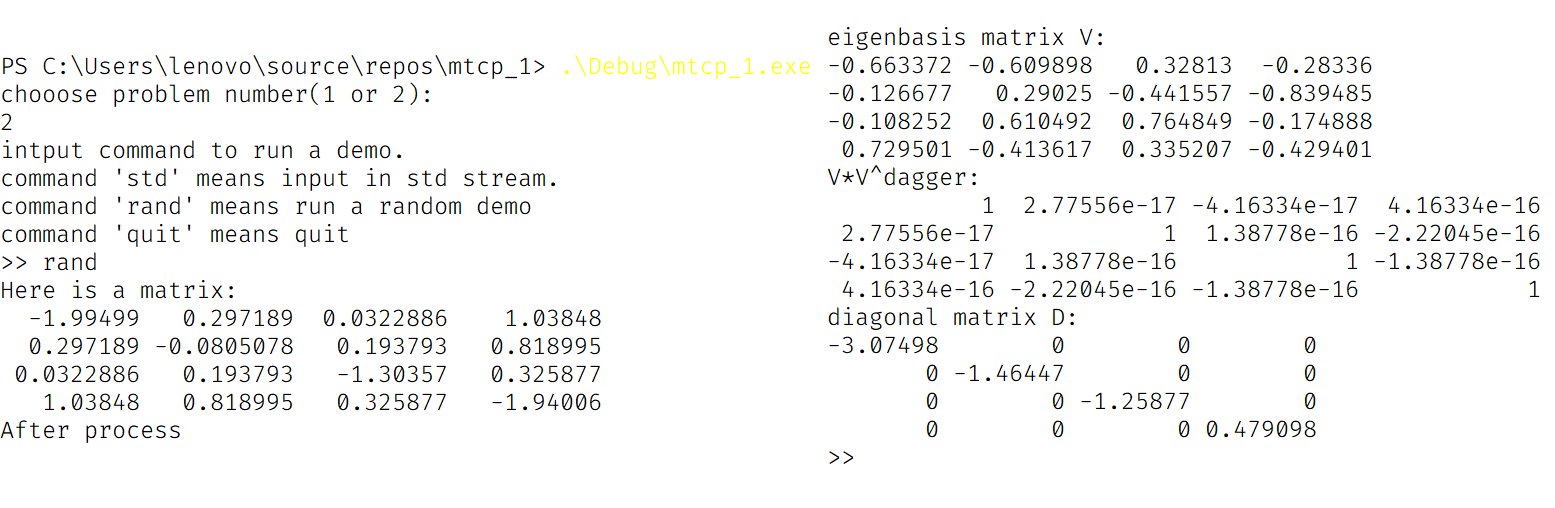
\includegraphics[width = 1.7\textheight]{img/result2.png}
        \caption{demo: input from random symetric matrix}
        \end{figure}
\end{frame}
